\documentclass[]{aiaa-tc} % insert '[draft]' option to show overfull boxes

 \title{Computing Automatic Analytic Gradients for Sparse Multidisciplinary Optimization in OpenMDAO}

\author{
  Tristan A. Hearn,%
     \thanks{Aerospace Engineer, MDAO Branch, Mail Stop 5-10, AIAA Member}
  \ Kenneth T. Moore,%
     \thanks{Senior Systems Engineer, MDAO Branch, Mail Stop 500-105, AIAA Senior Member}
  \ Justin Gray,%
     \thanks{Aerospace Engineer, MDAO Branch, Mail Stop 5-11, AIAA Member}
   \\
  {\normalsize\itshape
  NASA Glenn Research Center, Cleveland, OH}  \\
  John T. Hwang,%
  \thanks{Ph.D. Candidate, Department of Aerospace Engineering, AIAA Student Member}
  \ Joaquim R. R. A. Martins%
  \thanks{Associate Professor, Department of Aerospace Engineering, AIAA Associate Fellow}
  \\
  {\normalsize\itshape
   University of Michigan, Ann Arbor, MI}\\
  S. Andrew Ning
    \thanks{Senior Engineer, National Wind Technology Center, AIAA Member}
  \\
  {\normalsize\itshape
   National Renewable Energy Laboratory, Golden, CO}
}

\AIAAconference{Multidisciplinary Design Optimization Specialist Conference}
\AIAAcopyright{\AIAAcopyrightD{2012}}


% Define commands to assure consistent treatment throughout document
\newcommand{\eqnref}[1]{(\ref{#1})}
\newcommand{\class}[1]{\texttt{#1}}
\newcommand{\package}[1]{\texttt{#1}}
\newcommand{\file}[1]{\texttt{#1}}
\newcommand{\BibTeX}{\textsc{Bib}\TeX}

\setlength{\abovecaptionskip}{0pt}
\setlength{\belowcaptionskip}{0pt}

\usepackage{setspace}

\usepackage{graphicx}
\usepackage{wrapfig}
\usepackage{caption}
\usepackage{amsmath}
\usepackage{lscape}
\usepackage{hyperref}
\usepackage{minted}
\usepackage{color}
\usepackage{appendix}
\usepackage{listings}
\usepackage[section]{placeins}
\usepackage[superscript]{cite}
\usepackage{esdiff}
\usepackage{bm}

\lstset{frame=single}
\newcommand{\txt}{\textrm}


\captionsetup[figure]{margin=5pt,font=small,labelfont=bf,textfont=bf,justification=justified,}
%\captionsetup[wrapfigure]{margin=5pt,font=small,labelfont=bf,justification=justified,singlelinecheck=off}
\captionsetup[table]{margin=5pt,font=small,labelfont=bf,textfont=bf,justification=justified,position=top}

\bibliographystyle{aiaa}

\usepackage{lettrine}
\usepackage{verbatim}

\begin{document}

  \maketitle

  \begin{abstract}

  \end{abstract}

  \section{Introduction (Justin)}

    Gradient based optimization with analytic gradients is an effective tool for solving problems
    with large design spaces. It has been applied widely for aerodynamic shape optimization \cite{Liou2010,palacios2012adjoint}
    and structural optimization\cite{Kennedy:2013:TACS, Venkataraman:2004:SOC, Adelman:1986:structure-sensitivity}.
    In order to apply these methods to multidisciplinary problems, system level derivatives must be
    constructed by combining the partial derivatives from each discipline using the Global Sensitivity
    Equations\cite{Sobieski1990}. This technique is commonly applied to coupled
    aero-structural design optimization of aircraft wings\cite{Kenway2012c, Haghighat2012} and is applicable to
    other multidisciplinary design problems such as aero-acoustic design\cite{economon2012coupled}.Extending these
    gradient based techniques to more complex problem formulations has proved difficult. When
    design problems grow to include 10's of disciplines, it becomes increasingly difficult to construct the
    necessary derivatives. Even assuming all of the disciplines provide analytic partial derivatives,
    constructing the system level derivatives depends heavily on the structure of the data connections
    between disciplines. Manual implementations for these problems are time consuming and discourage modifications
    to the problem formulation in the future. To overcome this Moore developed a method for automatically assembling the system
    level derivatives based on the data-dependency graph of a given problem formulation\cite{openmdao_derivatives}. This
    work represented the first implementation of Martins and Hwang's unified approach to computing system level derivatives
    which combined forward and adjoint based derivatives into a single theoretical framework\cite{martins2013}. 
    In addition to allowing greater flexibility in the problem formulation, a key feature of Moore's graph-based approach, was the efficient
    handling of sparse problem formulations. By traversing the graph from design variables to quantities of interest,
    it was possible to consider only the subset of variables that were relevant to a specific system level gradient thus
    making gradient computations more efficient.

    Although Moore's work demonstrated that a framework could compute system level derivatives for arbitrary
    problem setups, the implementation assembled and inverted a complete system level Jacobian matrix for 
    all derivatives solves.  This made it unsuitable for larger problems involving 
    high-fidelity tools, since enumerating a full Jacobian would be inefficient (if possible at all).
    Hwang et. al. developed an alternative, graph-free, method for computing automatic system
    level sensitivities which used a global design variable vector\cite{CADRE2012}. Their method 
    addressed the scalability challenges with Moore's work by using a matrix-free approach with 
    components providing partial derivatives via a linear operator. They demonstrated the 
    effectiveness of their method on a design optimization of a small satellite
    with over 25,000 design variables and over 1 million state variables. Despite its success,
    the global-vector based approach required all the variables from the system model be
    included when solving for system level derivatives. This prevented their method
    from taking advantage of sparsity in the problem formulation and resulted in a less efficient gradient solving step.
    As a result, over 90\% of the compute effort was spent solving a linear system for the system
    level derivatives.

    This work combined the graph-based approach with the matrix-free solution algorithm
    to efficiently compute derivatives for a wide range of sparse, large-scale engineering
    design problems. We tested this new implementation on the same small satellite design problem used in 
    Hwang et. al's original work and demonstrated a dramatic reduction in computational cost. In addition
    this new method was applied to a wind turbine design study. This problem had a more 
    complex structure with stronger multidisciplinary couplings as well as a mixture of 
    analytic and finite difference gradients. Comparisons between finite-difference and analytic gradient 
    performance were made, demonstrating faster and tighter convergence with analytic gradients. 

  \section{Unified Derivatives Computations (John)}
  
	There are several methods for computing system-level derivatives that differ in accuracy, efficiency, and ease of implementation.
	The black-box finite-difference approximations involve the least amount of implementation effort, but they suffer from accuracy limitations that worsen with increasing nonlinearity in the model due to the combination of truncation and subtractive cancellation error.
	Furthermore, the cost is at best the number of design variables times the cost of evaluating the full multidisciplinary model.
	The complex-step method eliminates the accuracy issue at the cost of increased implementation complexity, but is typically two to three times slower than finite differences which is already relatively inefficient.
	
	The complex-step method can be invasive to a small extent, but the remaining methods typically require an even greater level of source code access and modification.
	Algorithmic differentiation (AD) uses automated tools to symbolically differentiate at the line-of-code level and combine the resulting partial derivatives to obtain numerically exact values for the system-level derivatives.
	AD operates in the forward and reverse modes, with the cost of the former proportional to the number of design variables and the latter to the number of output functions.
	Analytic methods have the same two modes of operation, and have the added advantage that only a linear system needs to be solved to obtain a vector of derivatives, which is cheaper than an evaluation of the model in some cases.
	
	When implementing multidisciplinary problems, derivatives for each individual discipline are typically available and must be combined to compute system-level derivatives.
	The manner in which the derivatives are combined is highly problem-dependent.
	If there is no feedback among the disciplines and they are explicit functions, one can simply use the chain rule at the discipline-level.
	If all of the disciplines have residuals from the discretization of governing equations, the coupled adjoint or coupled direct method would be the most appropriate for computing system-level derivatives.
	If the disciplines are explicit but there is coupling among disciplines, the GSE1 equations must be used.
	
	A framework that automatically computes system-level total derivatives from user-provided partial derivatives for each discipline must be able to apply the most appropriate method for the situation (explicit/implicit, coupled/sequential, etc.).
	This is greatly facilitated by a unification of derivative computation methods using a single equation from which all methods can be derived~[REF]:
	\begin{equation}
		\diffp[]{\bm C}{\bm v} \diff{\bm v}{\bm c} = \mathcal{\bm I} = \left. \diffp[]{\bm C}{\bm v} \right.^T \left. \diff{\bm v}{\bm c} \right.^T
	\end{equation}
	where $\bm C$ represents the vector of functions that constrain the variables $\bm v$ to their appropriate values.
	
	By appropriately choosing $\bm v$ and $\bm C$, the chain rule, black-box methods, analytic methods, the GSE1 equations, and algorithmic differentiation can be derived.
	For instance, including only the design variables and output variables in $\bm v$ yields a black-box method since all intermediate variables involved in computing the output variables are ignored in this situation.
	The significance of the above equation is that it enables a much simpler implementation of the derivative computation algorithm in the framework.
	Regardless of the specifics of a given problem, computing derivatives reduces to solving a linear system in the left or right equality of the above equation.

  \section{Dependency Graph (Ken/Justin)}\label{section:depgraph}

    In Moore's original work on computing derivatives from a dependency graph, he employed
    a discipline-based dependency graph, with a node for each discipline and edges describing
    dependency between the nodes. A path finding algorithm, from the NetworkX library\cite{hagberg-2008-exploring},
    computed the relevant set of disciplines for a given derivative. Although this took advantage of sparsity at
    one level, by excluding any disciplines that don't directly contribute, it didn't handle a second level of sparsity
    within disciplines. Even if a given discipline is relevant, some of its variables still may not 
    directly affect the quantities of interest. To handle this problem, Moore utilized a secondary source of information 
    outside the dependency graph. Pate et. al. proposed an alternative dependency graph
    structure that addressed this problem\cite{graph_problem2013}. Each discipline and each its variables are
    represented by separate nodes with directed edges between them describing their dependencies on each other.
    Figure \ref{fig:sellar_graph} shows a sample graph for the Sellar Problem \cite{AIAA:sellar}
    given in eqn. \ref{eqn:sellar_formulation}. This graph is essential for determining the set of relevant edges 
    for the gradient computation.

    \begin{align}
        \txt{given} & \ \ y_1 = D_1(x_1,y_2,z_1,z_2) \notag
        \\      & \ \ y_2 = D_2(y_1,z_1,z_2) \notag
        \\\txt{min.} &\ \ F(x_1,y_1,y_2,z_2) \notag
        \\\txt{w.r.t.} & \ \ x_1,y_1,y_2,z_1,z_2 \notag
        \\\txt{s.t.} & \ \ G_1(y_1) \geq 0 \notag
        \\     & \ \ G_2(y_2) \geq 0
        \label{eqn:sellar_formulation}
    \end{align}

    \begin{figure}[!htb]\begin{center}
      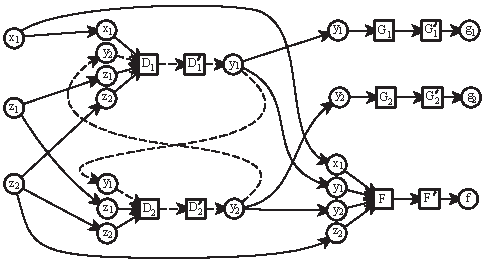
\includegraphics[width=.8\textwidth]{images/sellar_cycles}
      \caption{ Dependency graph for the Sellar problem. \label{fig:sellar_graph}}
    \end{center}\end{figure}

    In Pate et. al's graph syntax, a single node is given for every variable. This graph contains all the
    necessary information to take full advantage of problem sparsity, but suffers from one potential
    weakness. For a problem with millions of  variables, like the small satellite design problem,
    the graph would get very large and would be inefficient to operate on. To address this issue
    related variables, such as arrays, can be aggregated into a single node to represent the
    overall variable. If any specific sub-variable is referenced (e.g., some slice of an array).
    Figure \ref{fig:subvars} shows how the sub-variable nodes relate to their parent variables. Here,
    both outputs A.x and A.y are array variables. The full array A.x is connected to
    B.x while a single element of A.y is connected to the scalar B.z.

    \begin{figure}[!htb]\begin{center}
      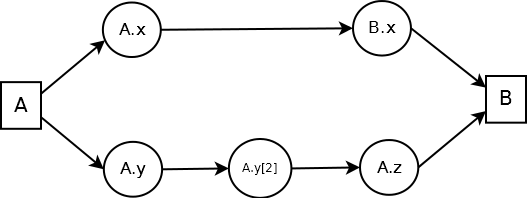
\includegraphics[width=.8\textwidth]{images/Graph1}
      \caption{ Example graph with child nodes for sub-variables \label{fig:subvars}}
    \end{center}\end{figure}

    By using the sub-variable nodes, the computational advantages of problem sparsity are retained. For example,
    consider $\frac{\partial B.z}{\partial A.y}$ from Fig. \ref{fig:subvars}. Given the graph, we know that
    this derivative will be sparse, with only $A.y[2]$ having non-zero values as in eqn.  \ref{eqn:sparse_gradient}.

    \begin{equation}
        \frac{\partial B.z}{\partial A.y} =
        \begin{bmatrix}
            0 \\
            0 \\
            \frac{\partial B.z}{\partial A.y[2]} \\
            \vdots \\
            0 \\
        \end{bmatrix}
        \label{eqn:sparse_gradient}
    \end{equation}

    When solving for derivatives, without the sub-var node, you would need to include all the
    elements of the $A.y$ array in the linear system for derivatives calculations.
    With the sub-var node, only the single relevant value from the array needs to be included.
    By representing hierarchical data as a single node, the overall size of the graph
    remains manageable, and the sub-var nodes are used to preserve the benefits of sparsity.


    \subsection{Graph Traversal Determining Relevance}

        OpenMDAO can calculate a gradient between any set of inputs and outputs nodes in a  
        model by setting up the appropriate linear system. The size of the linear system
        is determined by the number of variables being considered, which means that the linear
        system can get very large. Although the matrix-free approach to solving this system 
        can handle larger problems well, it is still desirable to minimize the size of the problem 
        as much as possible. OpenMDAO is able to achieve significant reductions in the
        size of the linear system by traversing the dependency graph to find the sub-set of relevant variables.
        For example, consider the notional graph in Fig. \ref{fig:graph2}. Considering $\frac{\partial Obj}{\partial param}$,
        the relevant components variables and components are highlighted. Only Components 1, 3, and 5 are needed.
        Furthermore only $C3.a$ is needed from Component 3, because of component level sparsity. 
        This means that only 4 variables are needed to solve for the derivatives, 
        instead of 7 if you did not reduce the graph. 

        \begin{figure}[!htb]\begin{center}
          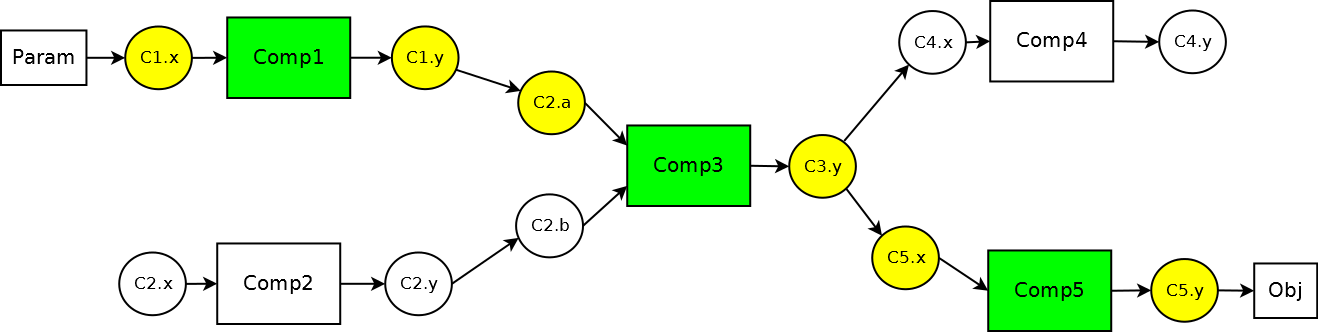
\includegraphics[width=.8\textwidth]{images/Graph2}
          \caption{ The reduced graph for the derivatives calculation includes Comps 1, 3,
          and 5 with their interconnecting variables. \label{fig:graph2}}
        \end{center}\end{figure}

        A traversal from parameter to quantity of interest, as shown in Fig. \ref{fig:graph2}, is used when solving for 
        forward derivatives. In forward mode, the traversal searches for all the variables that could possibly 
        be affected by a change in the parameter. One traversal is necessary for each design variable in the 
        problem formulation. To solve adjoint derivatives, a traversal must be made in 
        the opposite direction. In order to do this, simply reverse all the edges in the dependency graph and 
        perform one traversal from each quantity of interest to all possible parameters. 
        


    \subsection{Cycle Detection and Usage}
        Pate et. al indicate that within a dependency graph, the presence of cycles indicates coupling between
        the components in the cycle \cite{graph_problem2013}. Cycles can be induced by connections
        where data is passed directly from an output to an input, or implicitly where an input needs to
        be varied in order to drive a residual equation to zero. The presence of these cycles have 
        an impact on how models are solved. Firstly during normal execution, these cycles 
        need to be converged with a numerical solver such as Gauss-Seidel or Newton-based solver.
        In addition, these cycles need to be accounted for when solving for the derivatives. Martins and Hwang's 
        unified gradient method allows for this situation, but requires the resulting residual equations be
        handled in a slightly different manner from explicit variable relationships (ones without cycles). Hence 
        it is important to be able to efficiently identify all cycles in the graph. In formal terms, 
        cycles exist in a graph when a group of nodes are strongly connected. Tarjan's algorithm 
        applied to the dependency graph provides an efficient means of finding the sets of strongly 
        connected components\cite{tarjan1972depth,nuutila1994finding}. 


    \section{API for Specifying Discipline Derivatives (Tristan)}

        All of the discussion up to this point has dealt with disciplines as if they are black boxes
        which are assumed to provide analytic derivatives of their outputs with respect to their inputs
        to the framework. This section describes the api for components to declare and provide
        said derivatives. The api is broken up into two parts, one which is mandatory for all components
        that declare derivatives and a second which is optional for components that wish to take full
        advantage of the graph-based sparse approach.

        \subsection{Mandatory API Methods}

        There are 2 mandatory methods that all components supporting derivatives must provide.
        The first is \texttt{list\_deriv\_vars()}. This method specifies the
        input variables and output variables that make up the columns and rows of its Jacobian respectively.
        \texttt{list\_deriv\_vars()} returns a 2-tuple of inputs and outputs that have derivatives.
        A component is allowed to declare derivatives support for an arbitrary sub-set of all its variables.

        The second method is \texttt{provideJ()}. This method serves two purposes. First, it provides the
        opportunity to perform any one time work needed for linerization around the current point. Secondly,
        the method can optionally return the actual Jacobian, in the form of a $n \times m$ vector where $n$ is the
        number of outputs and $m$ is the number of inputs. The ordering of the rows and columns of the Jacobian
        must match the order of the variables returned for \texttt{list\_deriv\_vars()}. When a Jacobian is
        returned from \texttt{provideJ()}, OpenMDAO will cache it and use it for all derivative computations
        around the current point for both forward and adjoint derivatives. This makes the \texttt{provideJ()}
        API the most strait forward and easiest to use in many cases. Listing \ref{code:component_with_jacobian} shows
        an example of an OpenMDAO component with user-specified derivatives, using the provideJ method.
        This component has two input variables $x$ and $y$ and two output variables $f$ and $g$, where

        \begin{align}
            f\left(x, y\right) =&\  x^2 + \sin(y) \\ \notag
            g\left(x, y\right) =&\  x^3
        \end{align}

\begin{minipage}{\linewidth}
\begin{lstlisting}[label=code:component_with_jacobian,caption=Example OpenMDAO
component with user-specified Jacobian,
language=Python, basicstyle=\ttfamily\scriptsize,
           keywordstyle=\color{blue}\ttfamily,
           stringstyle=\color{red}\ttfamily, showstringspaces=false,
           commentstyle=\color{olive}\ttfamily]

from openmdao.main.api import Component
from openmdao.main.datatypes.api import Float
from math import sin, cos
from numpy import array

class ExampleComp(Component):

    # Inputs
    x = Float(0., iotype="in")
    y = Float(0., iotype="in")

    # Outputs
    f = Float(0., iotype="out")
    g = Float(0., iotype="out")

    def list_deriv_vars(self):
        return (('x', 'y',), ('f', 'g'))

    def provideJ(self):
        return array([[2 * self.x, cos(self.y)],
                      [3 * self.x ** 2, 0.0]])

    def execute(self):
        self.f = self.x ** 2 + sin(self.y)
        self.g = self.x ** 3

\end{lstlisting}
\end{minipage}

        Although the \texttt{provideJ()} method is easy to implement, it does have a few minor downsides. Firstly,
        it requires that the component Jacobian be assembled in memory. In most cases, with 10's or even 100's of variables
        this is reasonable but if the Jacobian has a sparse structure it may still be wasteful to allocate memory for a
        full matrix. Furthermore, for situations like CFD, where there are millions of variables spread out
        across many CPUs, assembling the full Jacobian is simply not feasible. Lastly, depending on how
        your problem is configured, it's possible that not all of the variables will be needed for a given problem as in Fig. \ref{fig:graph2}. 
        With \texttt{provideJ()} you still need to compute and provide the full Jacobian though some of it will be irrelevant.
        So in effect, using the \texttt{provideJ()} method can partially negate some of the benefits of problem sparsity. 
        In general these inefficiencies are small and easily outweighed by the easy of implementation. But in cases where 
        these downsides become a significant concern the \texttt{provideJ()} method should return nothing, and instead the
        optional API methods should be implemented for improved efficiency.

    \subsection{Optional API Methods}

        In order to overcome some of the downsides to construction of the full Jacobian, the components can provide
        a linear operator that computes the effect of multiplying the Jacobian with a given vector. This provides
        more freedom in how derivatives are implemented. It also enables the computing of only
        relevant quantities. The only significant downside is a small amount of added implementation complexity.
        Two different methods, \texttt{apply\_deriv(arg, result)} and \texttt{apply\_derivT(arg, result)}, must be implemented

        for forward and adjoint derivatives respectively. In each case, \texttt{arg} and \texttt{result}
        are dictionaries with relevant inputs and outputs variable names as keys.
        If you know you will be using only forward or adjoint, you can implement only the
        necessary method. Listing \ref{code:component_with_apply_deriv} provides an example of
        using the \texttt{apply\_deriv} and \texttt{apply\_derivT} methods, using the same component shown above in
        Listing \ref{code:component_with_jacobian}.

\begin{minipage}{\linewidth}
\begin{lstlisting}[label=code:component_with_apply_deriv,caption=Example OpenMDAO
component with apply\_deriv and apply\_derivT methods implemented,
language=Python , basicstyle=\ttfamily\scriptsize,
           keywordstyle=\color{blue}\ttfamily,
           stringstyle=\color{red}\ttfamily, showstringspaces=false,
           commentstyle=\color{olive}\ttfamily]

class ExampleComp(Component):

    # Inputs
    x = Float(0., iotype="in")
    y = Float(0., iotype="in")

    # Outputs
    f = Float(0., iotype="out")
    g = Float(0., iotype="out")

    def list_deriv_vars(self):
        return (('x', 'y',), ('f', 'g'))

    def provideJ(self):
        pass

    def apply_deriv(self, arg, result):
        if "x" in arg:
            result["f"] += 2 * self.x * arg["x"]
            result["g"] += 3 * self.x ** 2 * arg["x"]
        if "y" in arg:
            result["f"] += cos(self.y) * arg["y"]


    def apply_derivT(self, arg, result):
        if "f" in arg:
            result["x"] += 2 * self.x * arg["f"]
            result["y"] += cos(self.y) * arg["f"]
        if "g" in arg:
            result["x"] += 3 * self.x ** 2 * arg["g"]

    def execute(self):
        self.f = self.x ** 2 + sin(self.y)
        self.g = self.x ** 3

\end{lstlisting}
\end{minipage}

    The if conditions in the sample implementation from Listing \ref{code:component_with_apply_deriv} provide the
    mechanism for taking full advantage of sparsity. The usefulness of this feature can be readily demonstrated with
    a notional optimization using the Multidisciplinary Feasible architecture\cite{martins:arch:survey}.

    \begin{figure}[htbp]
        \centering
        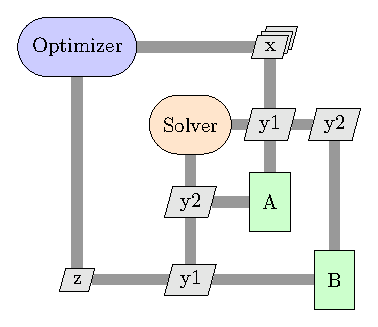
\includegraphics[width=0.5\textwidth]{xdsm/mdf_sample}
        \caption{Notional design problem with MDF problem formulation}
        \label{fig:MDF:XDSM}
    \end{figure}

    In fig. \ref{fig:MDF:XDSM}, the optimizer varies the design variable $A.x$, a large vector.
    The MDA converges variables $y_1$ and $y_2$ from disciplines $A$ and $B$. Applying a
    Newton-based method requires $\frac{\partial A.y_1}{\partial A.y_2}$ and $\frac{\partial B.y_2}{\partial B.y_1}$
    to converge, but $\frac{\partial A.y_1}{\partial A.x}$ is not. By using the linear operator derivatives method,
    the cost of multiplying by $\frac{\partial A.y_1}{\partial A.x}$ can be avoided while converging the MDA and only
    computed as part of the outer optimization loop.

    \section{Small Satellite Design Problem (Tristan)}

    CADRE (Cubesat investigating Atmospheric Density Response to Extreme driving)
    is a mission funded by the National Science Foundation to study the
    response of the thermosphere to auroral phenomena\cite{cutler2011cubesat}.
    The small satellite design problem optimizes the design of a cubsat for the CADRE mission.
    This problem was originally implemented and solved by Hwang et. al\cite{CADRE2012} using
    Martins and Hwang's matrix-free gradient strategy. The analysis models the orbit of a cubesat
    as it performs a mission over the course of a one year. The full mission is represented by
    by six half-days of operation, computed at conditions 1, 3, 5, 7, 9, and 11 months after launch.

    \begin{table}
        \centering
        \begin{tabular}{r l l l}
            \hline
            & Variable/function & Description & Quantity \\
            \hline
            maximize            & $\sum_{i=1}^6 D_i$ & Data downloaded \\
            \\
            with respect to & $0 \le I_\text{setpt} \le 0.4$ & Solar panel current & $300 \times 12 \times 6$ \\
                                    & $0 \le \gamma \le \pi / 2$ & Roll-angle profile & $300 \times 6$ \\
                                    & $0 \le P_\text{comm} \le 25$ & Communication power & $300 \times 6$ \\
                                    & $0 \le \text{cellInstd} \le 1$ & Cell vs. radiator & $84$ \\
                                    & $0 \le \text{finAngle} \le \pi / 2$ & Fin angle & $1$ \\
                                    & $0 \le \text{antAngle} \le \pi$ & Antenna angle & $1$ \\
                                    & $0.2 \le iSOC \le 1$ & Initial state of charge & $6$ \\
                                    & & Total & $25292$ \\
            \\
            subject to          & $I_\text{bat} - 5 \le 0$ & Battery charge constraint & $6$ \\
                                    & $-10 - I_\text{bat} \le 0$ & Battery discharge constraint & $6$ \\
                                    & $0.2 - SOC \le 0$ & Battery capacity constraint & $6$ \\
                                    & $SOC - 1 \le 0$ & Battery capacity constraint & $6$ \\
                                    & $fSOC - iSOC = 0$ & SOC periodicity constraint & $6$ \\
                                    & & Total & $30$ \\
            \hline
        \end{tabular}
        \caption{small satellite design problem formulation}
        \label{eqn:cadre_formulation}
    \end{table}

    The objective of the optimization was to maximize the total amount of data transmitted to the ground
    station, located in Ann Arbor, MI, over these six design points. There are 7 design varibles listed in Tabl. \ref{eqn:cadre_formulation}.
    3 of them, $\gamma$, $I_{setpt}$, and $P_{comm}$, are arrays of time varying schedules for the attitude,
    solar panel current, and communications power respectively. The remaining 4, $cellInstd$, $finAngle$, $antAngle$, $iSOC$,
    are all physical design variables of the satellite. All together there are 25,292 design variables.
    The 5 constraints for the problem relate to the battery charge rate, battery discharge rate,
    minimum battery capacity, maximum battery capacity, and a battery state-of-charge periodicity
    constraint. Each constraint is a length 6 vector with a value representing each of the 6 different
    orbits, yielding a total of 30 constraints. Since the problem has significantly more design
    variables than it does objectives and constraints, the problem was solved using adjoint gradients.

    \begin{figure}[!htbp]
        \centering
        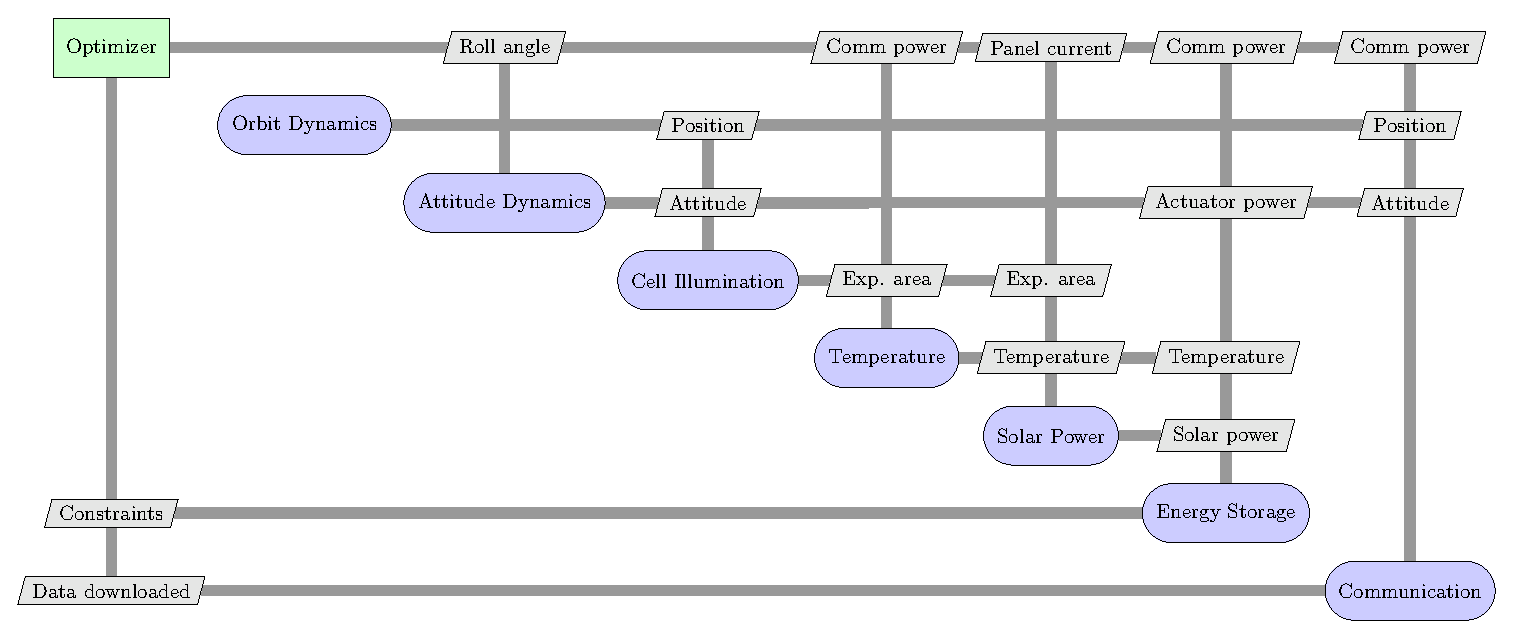
\includegraphics[width=0.95\textwidth]{xdsm/cadre_xdsm}
        \caption{XDSM diagram showing the structure of the small satellite design problem}
        \label{fig:cadre_xdsm}
    \end{figure}

    Overall the problem can be broken down into 7 distinct disciplines: orbit dynamics, attitude dynamics, cell illumination,
    temperature, solar power, energy storage, and communication. Figure \ref{fig:cadre_xdsm} shows how each of the disciplines
    relate to each other in the optimization problem. The actual implementation of the problem further
    subdivided most of the disciplines into smaller sub-disciplines. The true component level dependency
    graph, given in Fig. \ref{fig:cadre_graph}, has 39 different components. The full graph, including all variable and
    sub-variable nodes, is omitted for visual clarity.

    From a problem structure standpoint, this problem has three significant features. Firstly, the large number of
    disciplines, design variables, and the complex connections between them make assembling the linear system to solve for gradients
    challenging to do by hand. Secondly, although the problem does not have any explicit interdisciplinary coupling,
    there is coupling from the SOC periodicity constraint, $fSOC - iSOC = 0$, which is dependent on many of the
    disciplines. Thirdly, all disciplines were implemented with analytic derivatives so that no finite differencing was
    necessary.

    \begin{figure}[!htb]\begin{center}
      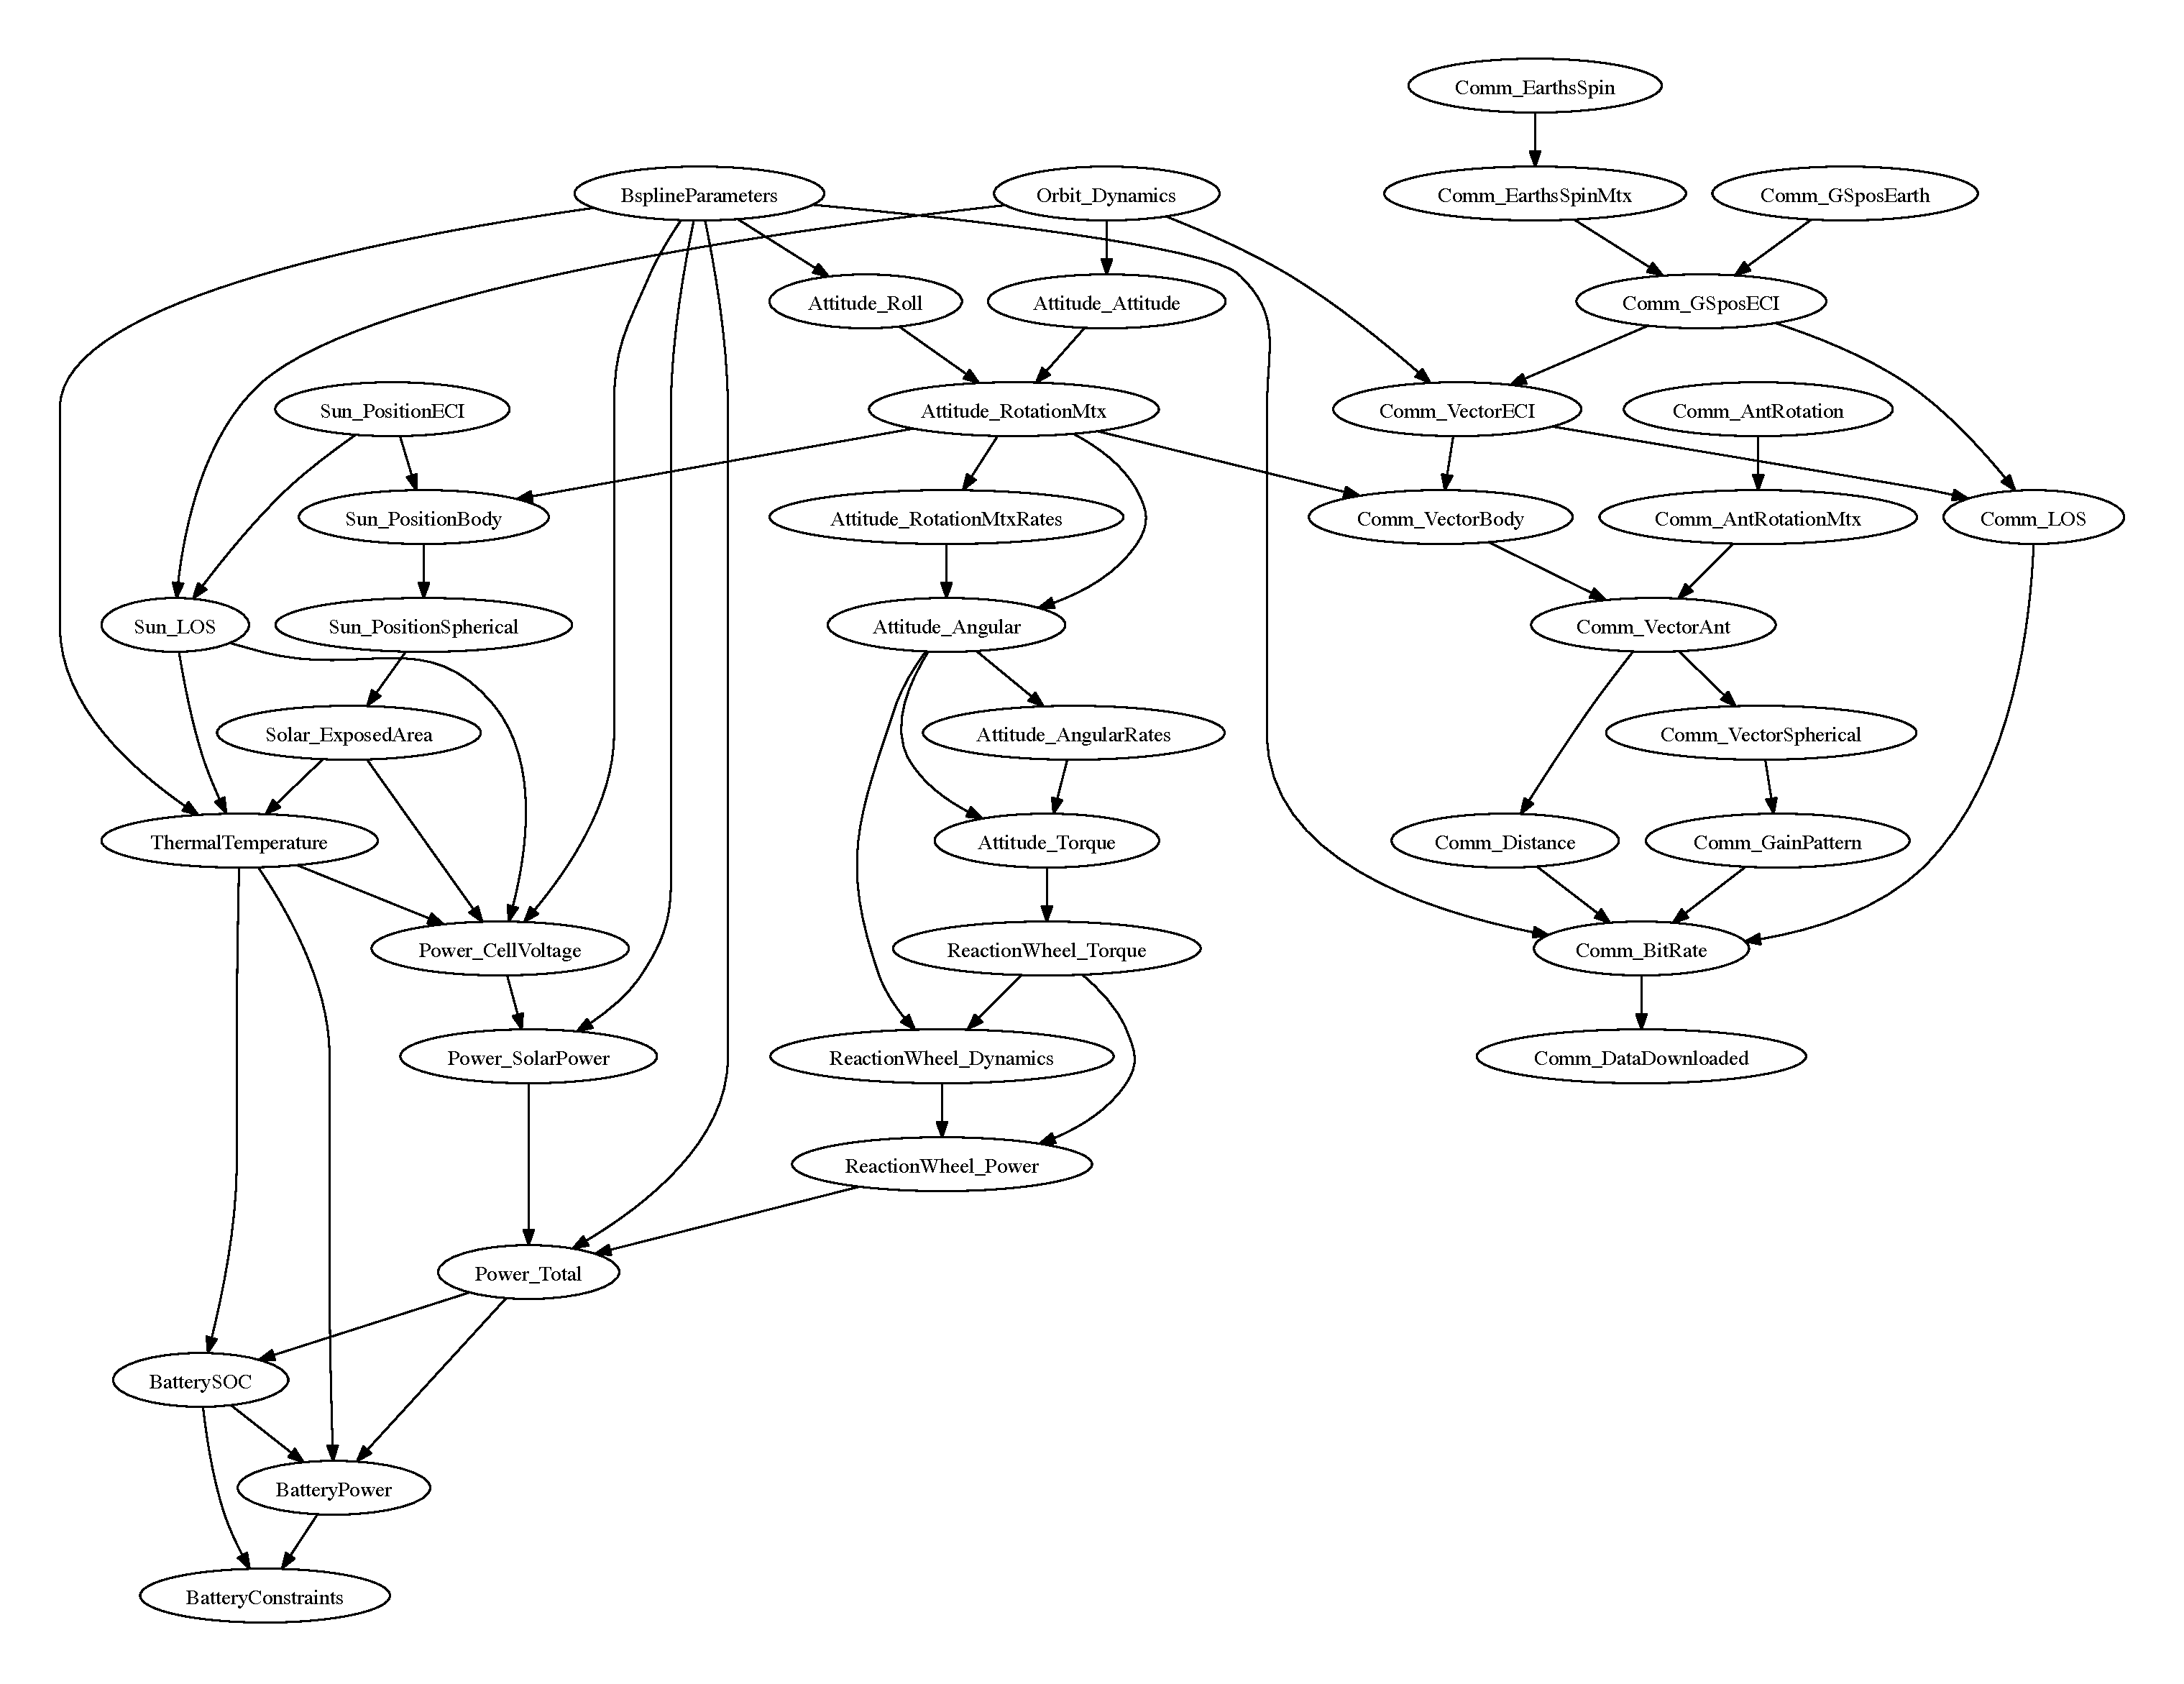
\includegraphics[width=.95\textwidth]{images/CADRE.pdf}
      \caption{ Dependency graph for the satellite problem. \label{fig:cadre_graph}}
    \end{center}\end{figure}

    \subsection{Optimization Results}


        \begin{figure}[!htb]
        \centering
        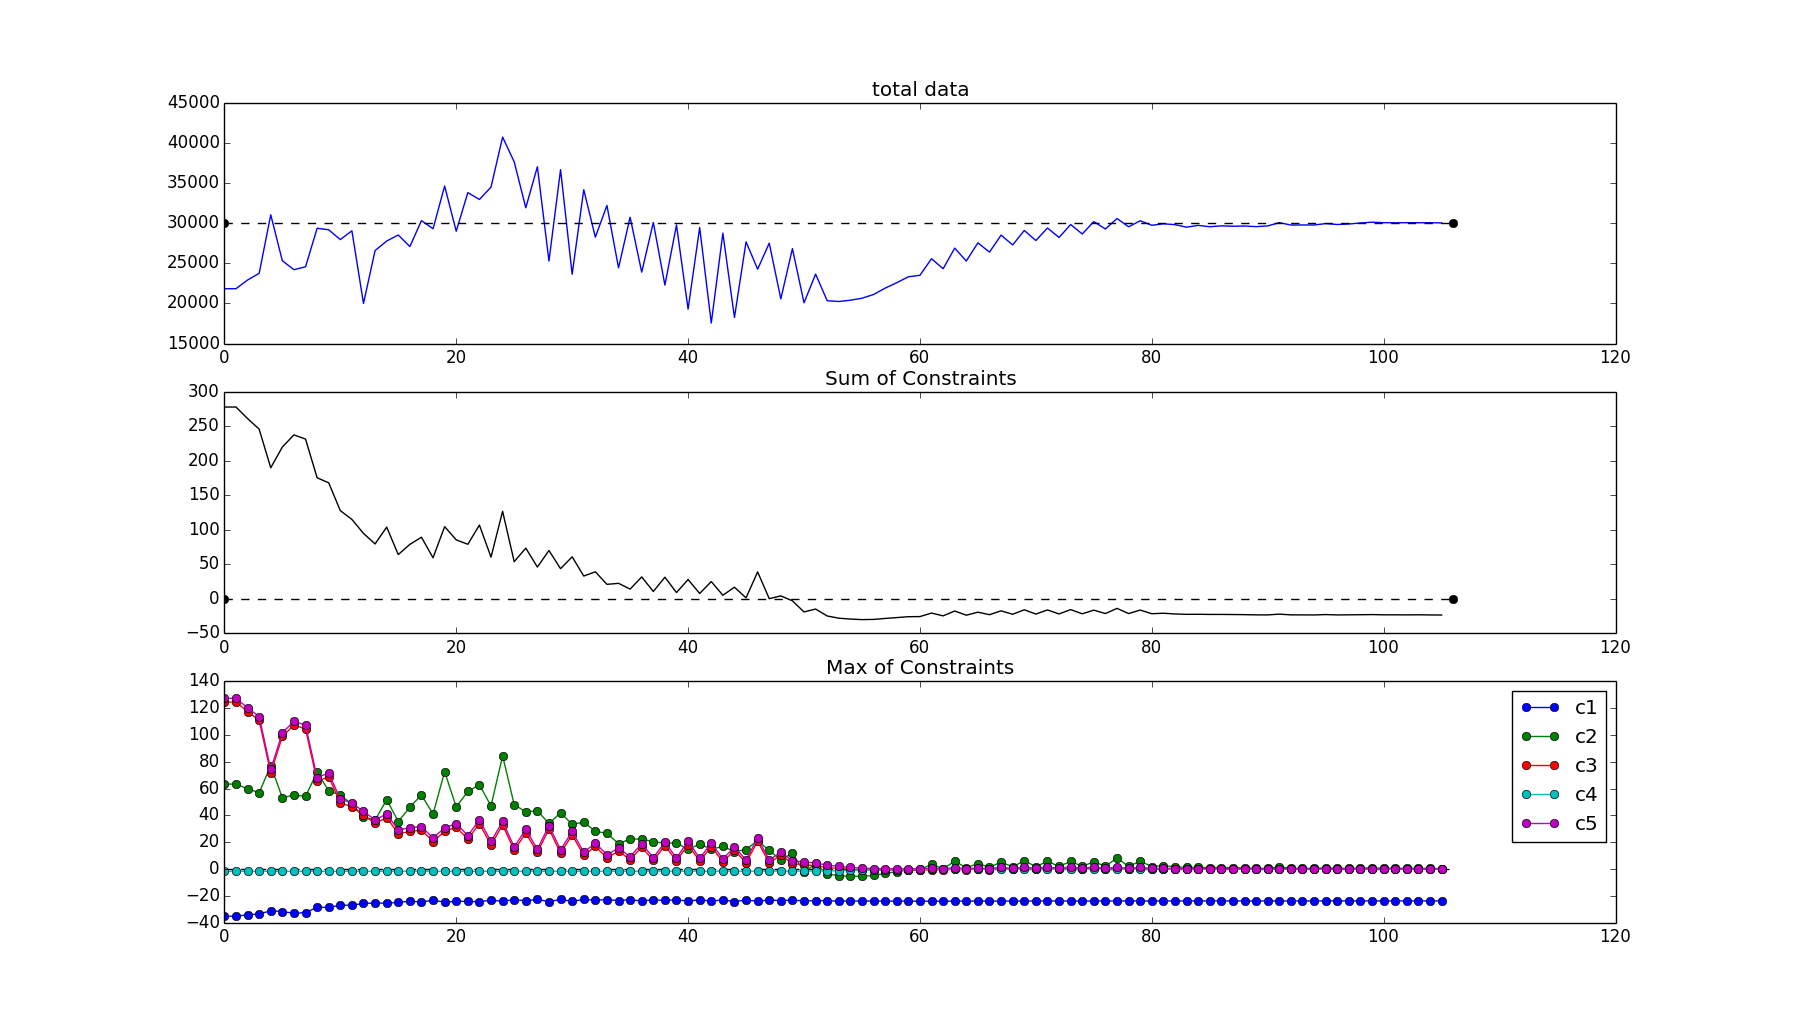
\includegraphics[width=0.99\textwidth]{images/opt}
        \caption[width=0.22\textwidth]{Convergence of the satellite problem.
        \label{convergence}
        }
        \end{figure}


        Figure \ref{convergence} illustrates the convergence of the satellite problem over the course of
        these iterations. The first row plots the
        value of the objective function, the total data downloaded over each design point. The objective
        function oscillated greatly over the course of the first half of the computed iterations, but
        stabilized by the 80th iteration at around the final optimum of about 3852 GigaBytes transfered.

        The second row plots the maximum value of each constraint across all design points at
        each iteration. As all of the problem constraint are non-positive for a feasible design,
        this can be taken as a cursory measure of overall problem feasibility.
        The third row plots the maximum value of each constraint across each of the design points,
        but separated according to specific constraint type. These two plots both indicate that the
        oscillatory behavior of the objective function coincided with a steady decrease in design
        infeasibility. Once a feasible state was reached (near the 50th iteration), the optimizer
        began refining the design towards a more favorable value of the objective function.

        \begin{figure}[!htb]
        \centering
        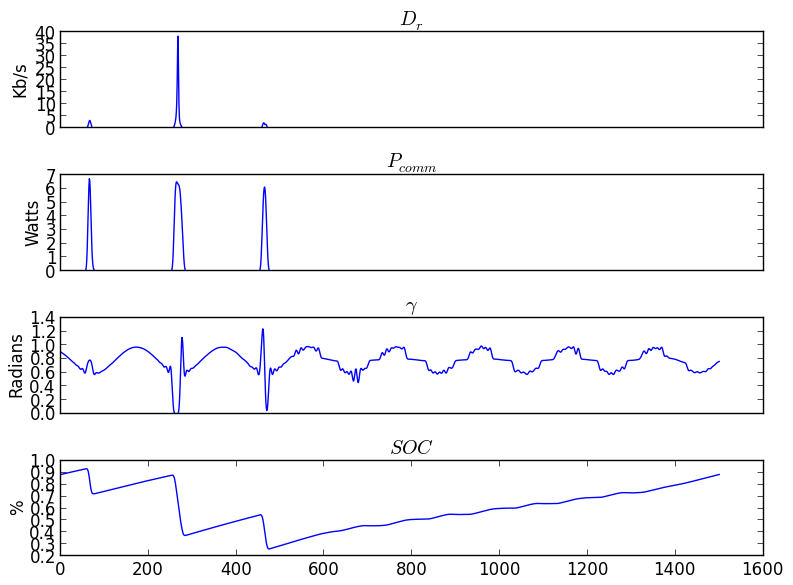
\includegraphics[width=0.8\textwidth]{images/pt_3_data}
        \caption[width=0.4\textwidth]{Plots of the bit rate, communications systems power, craft roll angle,
        and battery charge level over the half-day time period covered by the $4^{\textrm{th}}$ design point.
        \label{pt3_data_results}
        }
        \end{figure}

        Figure \ref{pt3_data_results} shows plots of selected variables for the $4^{\textrm{th}}$ design point,
        to illustrate the fidelity of the recovered solution. These variables are the communications
        bit rate ($D_r$), communications systems power level ($P_{comm}$), craft roll angle ($\gamma$),
        and battery charge level ($SOC$). Prior to the optimization, these variables
        were each instantiated to uniform values
        (across all time points) of 0, 0, $\frac{\pi}{4}$, and 0 respectively. The optimizer, operating on
        OpenMDAO's graph formulation of the problem succeeded at converging each of these variables to the values
        shown, for each time point. Line of sight is seen to have been achieved in three short ranges of time near the
        beginning of the modeled half-day design point. Interestingly, though the data rate achieved in the second
        time period with affirmative line of sight is significantly higher than the other two periods, the optimizer
        converged to a solution that provided power to the communications system near uniformly for each of these
        three time periods. This is likely due to the battery discharge rate and SOC constraints limiting
        the power which may be delivered to the communications system.

        Figure \ref{pt3_data_results} shows that the craft roll angle, $\gamma$, roughly approximates a sine function
        with a wavelength of 90 minutes (the approximate orbital period of the satellite),
        with short term perturbations during the time
        periods where line of sight is gained with the ground station. That is, the optimizer successfully
        converged to a solution with the satellite continuously turned to maximize exposure to the sun,
        except when turning to point its antenna towards the ground station during times when
        communication is possible. This dynamic is also reflected in the battery state of charge ($SOC$)
        data plotting in the bottom row, with the battery losing charge quickly during
        communication with the ground station, but recharging while tracking with the sun.

        Further post processing of the data included automatic geographical rendering of the trajectories of
        the  satellite for each of the 6 design points, using the Google
        Maps\footnote{http://developers.google.com/maps/} and Google
        Earth\footnote{http://developers.google.com/earth/} APIs. The trajectories are
        represented as polygonal chain ("polyline") elements, colored according to the
        satellites communication bit rate with the ground station during the corresponding
        window of time. Each colored line segment are centered on the locations
        determined by the time points when the data bit rate values were calculated
        by the OpenMDAO model.

         \begin{figure}[!htb]
            \centering
            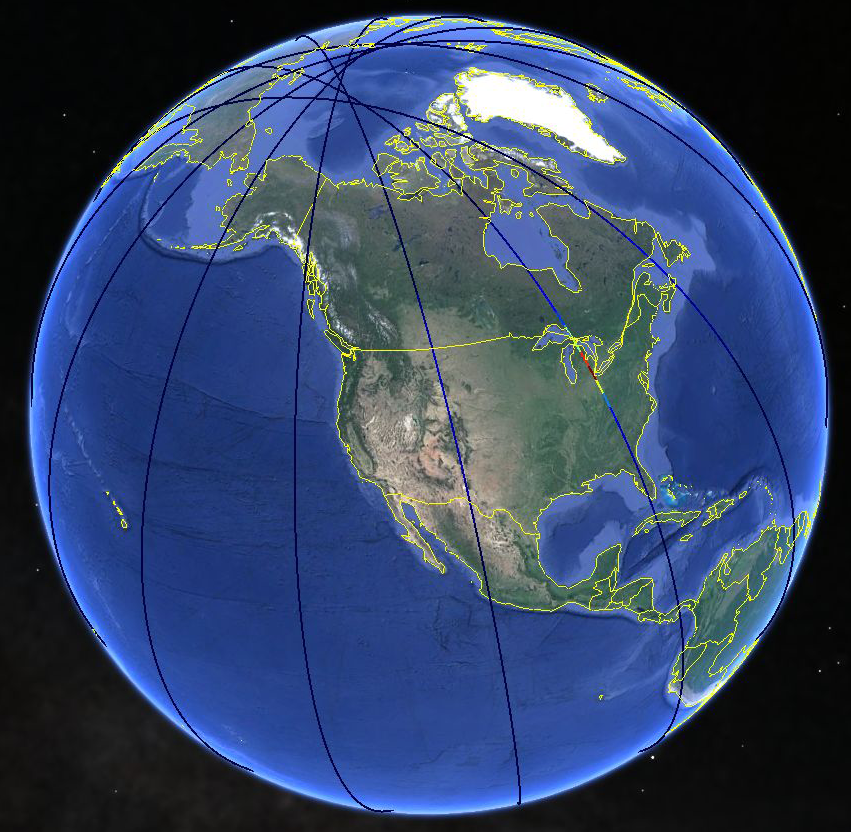
\includegraphics[width=0.49\textwidth]{images/pt3_gearth3}
            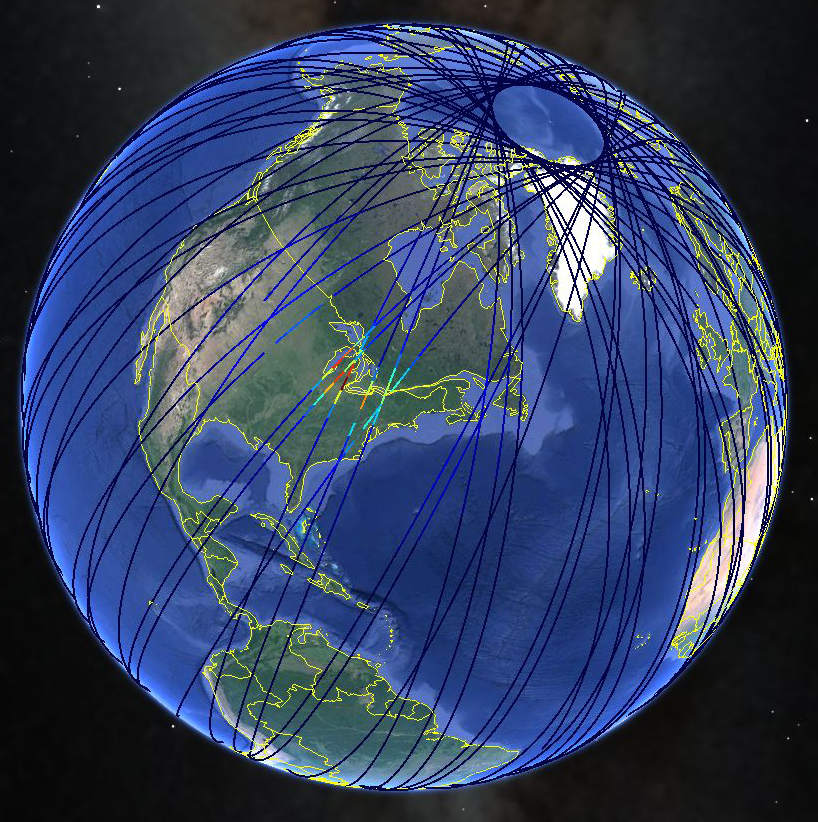
\includegraphics[width=0.49\textwidth]{images/allpts_gearth2}
            \caption{Plot of the trajectories of the satellite
            for the $4^{\textrm{th}}$ design point onto the surface of the Earth, illustrating the
            communication data rates near the ground station.
            \label{fig:trajectories1}
            }
        \end{figure}


        Figure \ref{fig:trajectories1} shows the communications bit rate along the trajectories of the
        satellite during the $4^{\textrm{th}}$ design point (left) and all points combined (right). 
        This can be compared directly with the data rate results in 
        Fig. \ref{pt3_data_results}, where one large spike in communications
        bit rate was preceded and then succeeded by two short time periods of lesser
        data rates. Plotted geographically, this is seen to be due to the procession of
        the satellites orbit, where the period of maximal data rate corresponds to a
        pass of the satellite directly over the ground station location. The proceeding and
        succeeding data rate spikes correspond to passes over the near Atlantic and
        Rocky Mountain regions, respectively.

       

        From Fig. \ref{fig:trajectories1} it's clear that the satellite is in a polar orbit. Since the
        goal of the optimization was to maximize data downloaded, we re-ran problem with the ground 
        station located at McMurdo Station, Antarctica because its position closer to the south poll 
        provided more opportunities to transmit data. The final optimal result gave 10340 GigaBytes
        transfered or about a 2.68X improvement. Fig \ref{fig:trajectories2} shows the ground trace 
        for this situation, clearly showing a much higher density of transmission situations. 

        \begin{figure}[!htb]
            \centering
            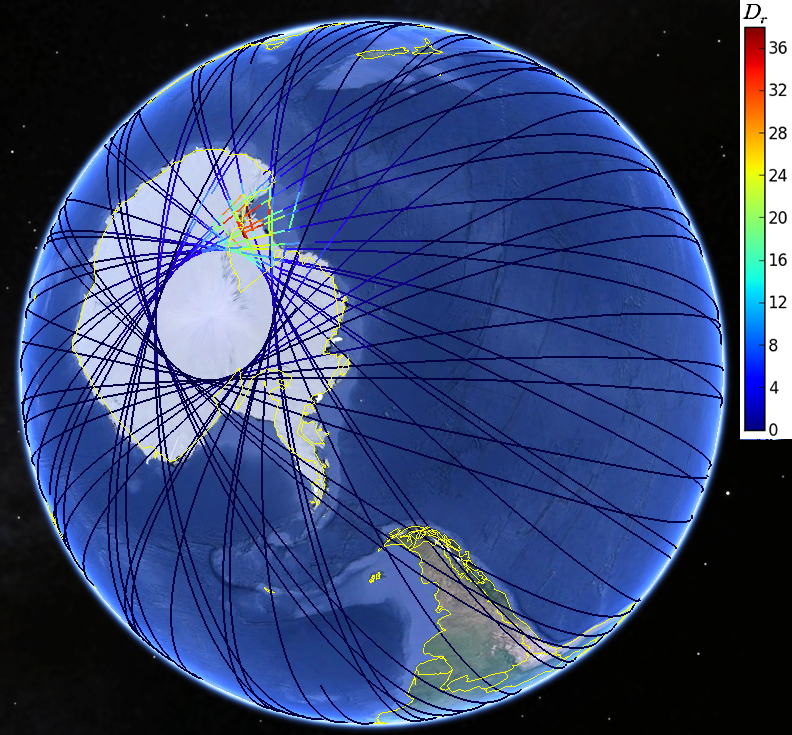
\includegraphics[width=0.49\textwidth]{images/allpts_gearth_mcmurdo}
            \caption{Plot of the trajectories of the satellite
            for the all design points onto the surface of the Earth, when the ground 
            station is at McMurdo Station, AntArctica. 
            \label{fig:trajectories2}
            }
        \end{figure}

        Figure \ref{fig:pt3_results_mcmurdo} provides the same selected variables as Fig. \ref{pt3_data_results}, 
        for this alternate case on the $4^{\textrm{th}}$ design point. The data shows how the optimizer is 
        able to handle the change in ground station and adjust the necessary schedules to re-optimize the 
        satellite. Notably there are now 5 different data transmission events compared to only 3 before. 


        \begin{figure}[!htbp]
            \centering
            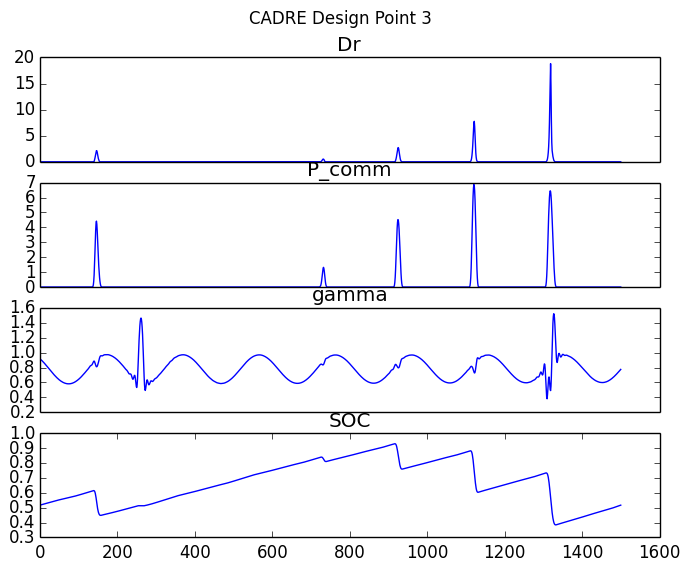
\includegraphics[width=0.5\textwidth]{images/cadre_results_mcmurdo}
            \caption{Plots of the bit rate, communications systems power, craft roll angle,
        and battery charge level over the half-day time period covered by the $4^{\textrm{th}}$ design point 
        with the ground station at McMurdo. }
            \label{fig:pt3_results_mcmurdo}
        \end{figure}


        \subsection{Performance Results}

            The OpenMDAO implementation of the satellite problem was executed on a
            Macbook Pro (2.3 Ghz Core i7 processor, 4GB 1600 Mhz DDR3 memory, running OSX 10.8.5). 
            The problem was converged to a termination tolerance of $10^{-5}$. This tolerance
            was achieved within approximately 106 iterations, using the SNOPT\cite{gill2005snopt}
            optimizer in about 6 hours. This represents a 16x improvement in computational
            cost compares to the original implementation by Hwang et. al. 


            Reduction of the derivative dependency graph, as discussed in
            Section \ref{section:depgraph}, is key for efficient execution
            of the CADRE problem; as there are a number of components which
            perform essential computations for the problem but do not have any influence
            on the fundamental design problem directly. For example, consider the orbital
            dynamics component, which computes the position and velocity of the satellite over
            time for each of the 6 design points. This component is not
            influenced by any of the design variables listed in Table \ref{eqn:cadre_formulation}. Therefore,
            there is clearly no need for this component to be executed more than once
            per design point, and the framework should exclude it from the
            derivatives dependency graph. However if the problem was
            reformulated to include, for example, selected orbital insertion parameters as
            design variables, then this would not be the case and the orbital
            dynamics component would not be excluded.

            Overall, without the reduction of the derivative graph the CADRE problem
            has 39 components with 64 edges. The total number of elements in
            the corresponding linear system is 358305. Average execution time
            for a single MDP case was 120 seconds.

            In contrast, when the derivative graph is automatically reduced based on
            relevance, the graph is reduced to 29 components with 45 edges.
            The corresponding linear system has 293792 (an 18\% reduction in
            problem size). Average execution time for a single case was
            72 seconds, a \% 40 reduction over the
            non-reduced problem.


  \section{Wind Turbine Design Problem (Justin/Andrew)}

    The goal of this design problem was to optimize a horizontal axis wind turbine to minimize the cost of energy. The problem considers the design of the rotor blades and tower from an aero-structural perspective as well as the structural requirements of the hub and nacelle.  Cost models for the turbine and wind plant are included to assess trade-offs in energy capture, capital costs and operational costs.  The analyses for this model are part of the Wind-Plant Integrated Systems Engineering \& Design Model (WISDEM) developed at NREL as part of a larger effort to develop a physics and cost based design optimization framework for wind turbines  \cite{Dykes2014a,Ning2013a,Ning2014,Ning2014d}

    A typical problem formulation is given in Tab.~\ref{tab:coe_formulation}.  Bound constraints were chosen to be large enough to not be active, except for those that must be restricted because of manufacturing or transportation reasons.  For simplicity, safety factors are not included in the list of constraints.


    \begin{table}
        \centering
        \caption{Horizontal axis wind turbine optimization problem description.}
        \begin{tabular}{r l l l}
            \hline
            & Variable/function & Description & Quantity \\
            \hline
            minimize            & $COE$ & Cost of energy \\
            \\
            with respect to & $0.4 \le c \le 20$ & Chord distribution & $5$ \\
                                    & $-10 \le \theta \le 30$ & Twist distribution & $4$ \\
                                    & $0.005 \le t_{sc} \le 0.2$ & Spar-cap thickness distribution & $5$ \\
                                    & $0.005 \le t_{te} \le 0.2$ & Trailing-edge panel distribution & $5$ \\
                                    & $3 \le \lambda \le 14$ & Tip-speed ratio in Region 2 & $1$ \\
                                    & $10 \le \lambda \le 80$ & Max Tip Speed & $1$ \\
                                    & $40 \le L_{blade} \le 100$ & Blade length & $1$ \\
                                    & $0.1 \le L_{shaft} \le 10$ & Low speed shaft lengths & $2$ \\
                                    & $0.01 \le h_{beam} \le 10$ & Bedplate I-beam sizing & $2$ \\
                                    & $3.87 \le d \le 20$ & Tower diameter & $3$ \\
                                    & $0.005 \le t \le 0.2$ & Tower wall thickness & $3$ \\
                                    & $0.25 \le z_{waist} \le 0.75$ & Tower waist location & $1$ \\
                                    & $50 \le H \le 200$ & Tower height & $1$ \\
                                    & & Total & $34$ \\

            \\
            subject to          & $\delta_{tip} \le \delta_{max}$ & Blade tower strike & $1$ \\
                                    & $\delta_{ground} \ge \delta_{min}$ & Blade ground clearance & $1$ \\
                                    & $\epsilon \le \epsilon_{ult}$ & Ultimate strain in blades & $24$ \\
                                    & $\epsilon \le \epsilon_{cr}$ & Panel buckling in blades & $14$ \\
                                    & $damage \le 1$ & Fatigue damage in blades & $10$ \\
                                    & $\delta_{lss} \le \delta_{max}$ & Deflection limits in low-speed shaft & $4$ \\
                                    & $\delta_{bdp} \le \delta_{max}$ & Deflection limits in bedplate & $2$ \\
                                    & $\sigma_{bdp} \le \sigma_{ult}$ & Ultimate stress in bedplate & $2$ \\
                                    & $\sigma_{twr} \le \sigma_{ult}$ & Ultimate stress in tower & $14$ \\
                                    & $\sigma_{twr} \le \sigma_{shell}$ & Shell buckling in tower & $14$ \\
                                    & $\sigma_{twr} \le \sigma_{global}$ & Global buckling in tower & $14$ \\
                                    & $damage \le 1$ & Fatigue damage in tower & $9$ \\
                                    & $f \ge \Omega_{rotor}$ & Tower resonance avoidance & $1$ \\
                                    & $d/t \ge 120$ & Weldability & $1$ \\
                                    & $d_{top}/d_{base} > 0.4$ & Manufacturability & $1$ \\
                                    & & Total & $112$ \\
            \hline
        \end{tabular}
        \label{tab:coe_formulation}
    \end{table}


    There are 34 design variables, 1 objective, and 112 constraints. Since there are
    less design variables then quantities of interest, the problem was solved with
    forward derivatives. In addition, the relatively small size of the design space
    enabled the use of both analytic and finite difference gradients. There are 10 disciplines 
    involved in the top level of the model, as seen in Fig.~\ref{fig:xdsm_wt}. Similar to the small 
    satellite design problem, many of the disciplines were further
    sub-divided into more than one component for implementation. However, in the
    satellite problem, all components were left at the same level in the model. For this problem, 
    actual sub-assemblies of components were made, adding a layer of abstraction. Rotor, 
    Hub, Nacelle, Tower, Turbine Capital Cost, and Balance of Station are all 
    assemblies with significant internal structures. This highly nested model structure was 
    designed to support modularity in the model, to allow a wide range or researchers to build 
    discipline models swap them in and out of the overall model. The presence of these 
    sub-assemblies is important to how the derivatives are computed. The assemblies are
    treated as an atomic discipline form the perspective of the top-level model. This means that
    when derivatives are requested from the assembly, it will internally solver for its own 
    boundary derivatives and report them to the top level assembly. 

    The Rotor discipline in particular has a very complex structure, including some internal 
    iterations on the PowerCurve component. 

    The presence of these sub


    \begin{figure}[!htbp]
        \centering
        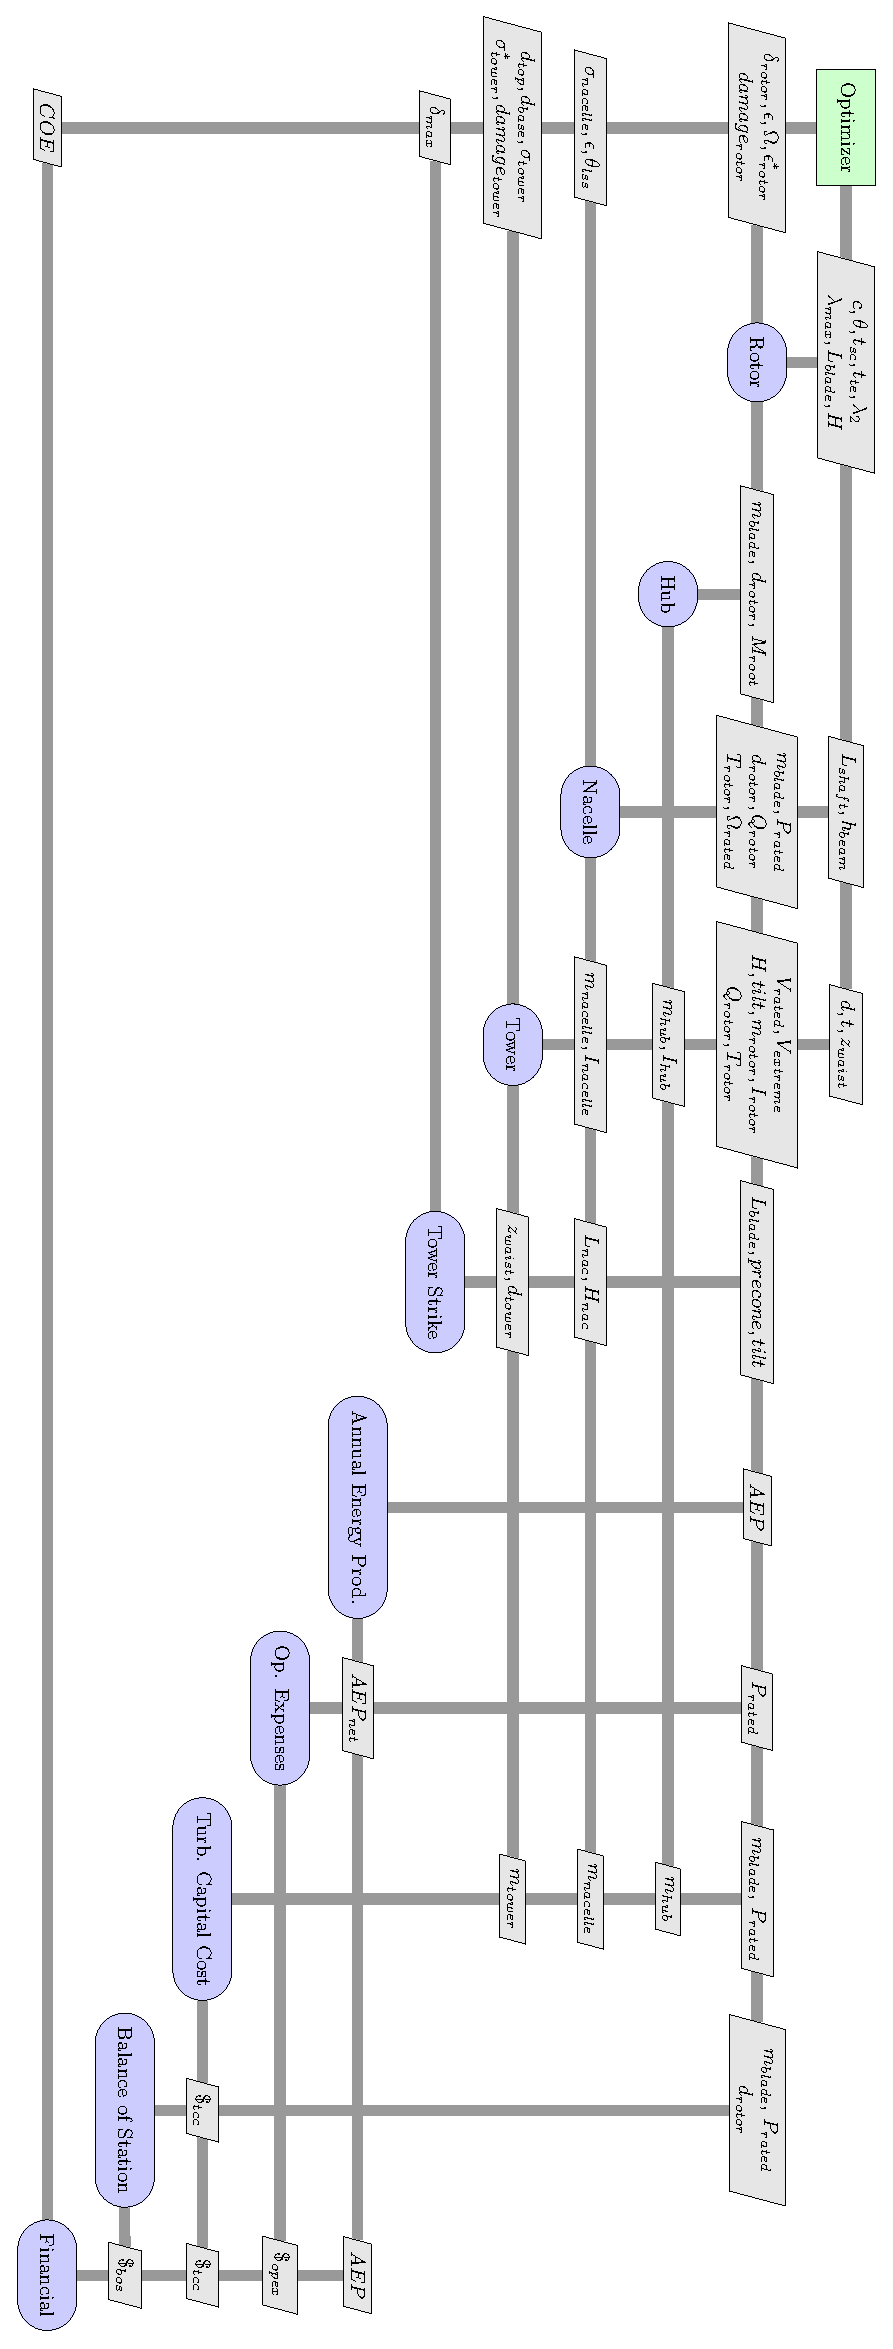
\includegraphics[width=0.95\textwidth]{xdsm/wt_xdsm}
        \caption{XDSM diagram of the wind turbine design optimization}
        \label{fig:xdsm_wt}
    \end{figure}

    The rotor aerodynamics discipline is modeled with a blade element momentum (BEM)
    tool, CCBlade\cite{NING:BEM}. The use of CCBlade is significant because it implements
    a BEM implementation specifically tailored to optimization.  Tower aerodynamics was 
    modeled with assumed power-law wind profiles, and cylinder drag theory.
    The structures discipline for the blades was modeled with pBEAM \cite{Ning2013b},
    a beam finite element code, PreComp \cite{Bir2005}, a structural property tool for
    composite blades, and additional structural modules for panel buckling and fatigue.
    Tower structures is modeled with pBEAM, and additional modules for shell buckling,
    global buckling, and fatigue.  Some drivetrain components were modeling with scaling
    relationships (bearings, yaw system, generator), while others were bottom-up physics
    models (bedplate, gearbox, low-speed shaft).

     For this
    problem the components representing the XXX and YYY disciplines were
    grouped into sub-assemblies. Figure \ref{fig:wt_top_depgraph} shows the
    top level dependency graph for the problem. The XXX discipline assembly dependency
    graph is in Fig. \ref{fig:wt_sub_depgraph} shows the internal configuration
    of components, as well as their links to the top level model.

    \begin{figure}[!htbp]
        \centering
        [Insert Top Level Dependency Graph]
        %\includegraphics[width=0.95\textwidth]{}
        \caption{Wind turbine problem top level dependency graph}
        \label{fig:wt_top_depgraph}
    \end{figure}

    \begin{figure}[!htbp]
        \centering
        [Insert Sub-Assembly Dependency Graphs]
        %\includegraphics[width=0.95\textwidth]{}
        \caption{Sub-assembly XXX dependency graph}
        \label{fig:wt_sub_depgraph}
    \end{figure}


    This problem has one additional interesting characteristic with regards to its
    problem formulation. It has a number of data connections throughout the dependency
    graph which are never relevant to the derivatives calculations. These non-relevant
    variables are used for various settings and initialization values throughout the
    model, such as the number of blades on the rotor or the density of air. 
    Such variables, especially when they are integers (or otherwise non-differentiable)
    necessitate the graph based approach to identifying irrelevant variables. Without that, these
    variables would be included in the linear systems for derivatives causing erroneous
    results. 


    \subsection{Results}
        \begin{itemize}
            \item FD vs analytic results
            \item speed issues without directional derivatives
        \end{itemize}


  \section{Conclusion (Justin/Tristan)}

      This work demonstrates how a graph-based approach to problem formulation compliments and enhances the benefits of gradient based
      optimization. The graph provides a proper structure to handle the necessary bookkeeping to automatically implement complex
      problem formulations while making use of analytic gradients. By implementing this graph based approach in OpenMDAO, the framework
      can alleviate the responsibilities for such bookkeeping from the user entirely which dramatically simplifies implementation.

      The two problems examined in this work demonstrate that a single framework can operate efficiently and effectively on a wide range of large-scale problems.

  \bibliography{references}


\end{document}
